% ---------------------------------------------------------------------------
% Replication exercise: India's National Tobacco Control Programme
% Self-contained: compiles on Overleaf with no other files except trends.png.
% ---------------------------------------------------------------------------
\documentclass[11pt,a4paper]{article}

\usepackage[T1]{fontenc}
\usepackage[utf8]{inputenc}
\usepackage{lmodern}
\usepackage[margin=1in]{geometry}
\usepackage{amsmath}
\usepackage{booktabs}
\usepackage{graphicx}
\usepackage{listings}
\usepackage{xcolor}
\usepackage{enumitem}
\usepackage{tcolorbox}

\definecolor{NavyBlue}{HTML}{1F3A68}
\definecolor{CodeBg}{HTML}{F6F7F9}
\definecolor{OutBg}{HTML}{FFFDF5}
\definecolor{Rule}{HTML}{C9CED6}

\usepackage[colorlinks=true,linkcolor=NavyBlue,urlcolor=NavyBlue]{hyperref}

\lstdefinestyle{rcode}{
  basicstyle=\ttfamily\footnotesize,
  backgroundcolor=\color{CodeBg},
  frame=single, framerule=0.4pt, rulecolor=\color{Rule},
  breaklines=true, columns=fullflexible, keepspaces=true,
  xleftmargin=0pt, framexleftmargin=4pt, framexrightmargin=4pt,
  aboveskip=0.9em, belowskip=0.9em,
  commentstyle=\color{NavyBlue!70}, language=R
}
\lstdefinestyle{rout}{
  basicstyle=\ttfamily\scriptsize,
  backgroundcolor=\color{OutBg},
  frame=single, framerule=0.4pt, rulecolor=\color{Rule},
  breaklines=false, columns=fullflexible, keepspaces=true,
  xleftmargin=0pt, framexleftmargin=4pt, framexrightmargin=4pt,
  aboveskip=0.9em, belowskip=1.2em
}
\lstset{style=rcode}

\newcommand{\Rin}[1]{\lstinputlisting[style=rcode]{#1}}

\newtcolorbox{notebox}[1]{
  colback=NavyBlue!4, colframe=NavyBlue!55, boxrule=0.5pt,
  left=8pt, right=8pt, top=6pt, bottom=6pt,
  before upper={\setlength{\parskip}{0.6em}},
  title={\footnotesize\bfseries #1}, fonttitle=\normalfont
}

\setlength{\parskip}{0.55em}
\setlength{\parindent}{0pt}

\newcommand{\qhead}[1]{\subsection*{#1}\addcontentsline{toc}{subsection}{#1}}

\title{\bfseries Did India's Tobacco Control Programme Work?\\[0.3em]
       \large A replication exercise in difference-in-differences}
\author{Kedar Kulkarni}
\date{}

\begin{document}
\maketitle
\thispagestyle{empty}

\begin{notebox}{What you are replicating}
Nazar GP, Chang KC-M, Srivastava S, Pearce N, Karan A, Millett C (2020).
\emph{Impact of India's National Tobacco Control Programme on bidi and
cigarette consumption: a difference-in-differences analysis.}
\textbf{Tobacco Control} 29:103--110.

India launched the National Tobacco Control Programme (NTCP) in 42 districts
between 2007 and 2009. The paper asks whether household tobacco consumption
fell in those districts relative to the rest of the country, using three
rounds of the NSS Consumer Expenditure Survey: round 55 (1999--2000), round 61
(2004--05) and round 68 (2011--12). Its answer is \textbf{no}.
\end{notebox}

\section*{Why this exercise}

Most of what you have seen about difference-in-differences has been about
getting the estimate right. This exercise is about something else: what it
feels like to run a credible design and find nothing.

The paper's conclusion is a null. That is not a failed study. A programme
reaching 42 districts, evaluated against 850-odd control districts over
twelve years, that moves no measurable outcome is a real and publishable
finding about the programme. But a null is also exactly what you get from a
design that is too noisy to detect anything, and part of your job here is to
tell those two apart.

You are given a cleaned file. The merging and the district concordance --- the
part of the original replication that took far longer than the regressions ---
have been done for you. One thing to carry away anyway: the three NSS rounds
do not share a state coding scheme, do not share item codes for bidi and
cigarettes, and do not use the same district names. Uttar Pradesh is state 25
in round 55 and state 09 in rounds 61 and 68. Bidi is item 320 in rounds 55
and 61 and item 310 in round 68; read round 68 with 320 and you silently get
ganja. Of the paper's 42 treated districts, only 21 could be matched
unambiguously across all three rounds, and those 21 are the treatment group
here.

\section*{The data}

\texttt{ntcp.rds} holds 346{,}602 households across the three rounds. Each row
is one household in one round. There is no household panel: the NSS draws a
fresh sample each round.

\begin{center}
\footnotesize
\begin{tabular}{@{}llp{8.1cm}@{}}
\toprule
\textbf{Variable} & \textbf{Type} & \textbf{What it is} \\
\midrule
\texttt{hhid}        & chr  & household identifier \\
\texttt{round}       & num  & 55, 61 or 68 \\
\texttt{year}        & fct  & 1999-2000, 2004-05, 2011-12 \\
\texttt{period}      & fct  & \texttt{pre}, \texttt{pre2}, \texttt{post} \\
\texttt{t2}          & int  & 1 in 2004-05, else 0 \\
\texttt{t3}          & int  & 1 in 2011-12, else 0 \\
\texttt{ntcp}        & int  & 1 if the district is one of the 21 NTCP districts \\
\texttt{state\_code} & num  & NSS state code, \emph{as coded in that round} \\
\texttt{dist\_code}  & num  & NSS district code, \emph{as coded in that round} \\
\texttt{urban}       & int  & 1 if urban \\
\texttt{hh\_size}    & num  & number of persons \\
\texttt{mpce}        & num  & monthly per capita consumption expenditure, Rs. \\
\texttt{wealth\_q}   & int  & quintile of log \texttt{mpce} \emph{within round} \\
\texttt{wgt}         & num  & survey weight (not used below) \\
\texttt{bidi\_sticks}& num  & bidis consumed, 30-day recall \\
\texttt{cig\_sticks} & num  & cigarettes consumed, 30-day recall \\
\texttt{any\_bidi}   & int  & 1 if \texttt{bidi\_sticks} $>$ 0 \\
\texttt{any\_cig}    & int  & 1 if \texttt{cig\_sticks} $>$ 0 \\
\bottomrule
\end{tabular}
\end{center}

Two variables you will need are deliberately absent. Build them yourself.

\begin{notebox}{The specification}
Both parts of the model carry the same structure, with 1999--2000 as the base
period:
\[
  y = \beta_0 + \beta_1\,\text{NTCP} + \beta_2 t_2 + \beta_3 t_3
      + \underbrace{\delta_1 (\text{NTCP}\times t_2)}_{\text{DID1}}
      + \underbrace{\delta_2 (\text{NTCP}\times t_3)}_{\text{DID2}}
      + \mathbf{X}\gamma
\]
\textbf{DID2} is the estimate of interest: NTCP districts against controls,
after the programme.

\textbf{DID1} compares 2004--05 with 1999--2000. \emph{Both precede the
programme.} Under parallel trends it should be zero, so DID1 is a falsification
test, not a result. Report it before you report DID2.

The paper uses a \textbf{two-part model}, because most households consume no
tobacco at all and the rest are heavily right-skewed:
part 1 is a logit for whether the household consumes at all; part 2 is a linear
regression of log sticks per person among households that do.
\end{notebox}

\clearpage
\section*{Questions}

Work in R. Standard errors should be clustered on district throughout
(\texttt{sandwich::vcovCL}), since treatment is assigned at the district level.

\begin{enumerate}[label=\textbf{Q\arabic*.},leftmargin=*,itemsep=0.7em]

\item Load \texttt{ntcp.rds}. How many households are there in each round, and
how many are in NTCP districts? Then count the distinct treated and control
districts. Count them \emph{within each round} and explain why pooling the
rounds gives the wrong answer.

\item Are these data a panel? Answer it with the data, not from memory, and say
what the answer rules out --- which estimators are now unavailable to you.

\item Report the share of households consuming any bidi and any cigarettes, by
year and by treatment group. Before doing anything else, read the six numbers
for bidi. What do they already tell you about the design?

\item Compute the bidi-prevalence difference-in-differences by hand from the
$2\times2$ table of means (1999--2000 versus 2011--12). Write down the change
in the treated group, the change in the control group, and the difference.

\item Reproduce the same number as a regression coefficient using a linear
probability model on the two end rounds only. Which coefficient is the DiD?

\item Now use all three rounds and add controls: \texttt{urban},
\texttt{log(hh\_size)}, wealth quintile and state fixed effects, with
district-clustered standard errors. Compare the \texttt{ntcp:t3} coefficient
with your answer to Q4 and account for the difference in both the point
estimate and the standard error.

\item Estimate part 1 of the paper's model: a logit for \texttt{any\_bidi} with
the same controls. Report DID1 and DID2 as odds ratios with 95\% confidence
intervals.

\item Estimate part 2: construct log bidi sticks per person and regress it on
the same specification among consuming households only. Report DID1 and DID2.
What does conditioning on consumption do to the interpretation of this
coefficient?

\item State the pre-trend test in words, give its value, and say what you
conclude. Then say what the \emph{width} of its confidence interval tells you,
separately from whether it contains 1.

\item Repeat Q7 for cigarettes. You will find something the paper did not.
Before calling it a finding, list the differences between this replication and
the paper that could produce it.

\end{enumerate}

\begin{notebox}{For the write-up}
Three of the paper's four estimates reproduce here as nulls, and the fourth
does not. Write a paragraph a referee would accept on whether this replication
supports the paper's conclusion. The honest answer involves the phrase
``cannot distinguish''.
\end{notebox}

\clearpage
\section*{Solutions}

All output below comes from running \texttt{solutions.R} on
\texttt{ntcp.rds}. Numbers are unweighted throughout.

% ---------------------------------------------------------------------------
\qhead{Q1. The data}

\begin{lstlisting}[style=rcode]
ntcp <- readRDS("ntcp.rds")
dim(ntcp)
table(year = ntcp$year, treated = ntcp$ntcp)
\end{lstlisting}

\begin{lstlisting}[style=rout]
[1] 346602     18
           treated
year             0      1
  1999-2000 112854   7455
  2004-05   118923   5719
  2011-12    97241   4410
\end{lstlisting}

The treated group is small: between 4{,}400 and 7{,}500 households per round,
against roughly 100{,}000 controls. Keep that asymmetry in mind --- it is where
the precision of every estimate below comes from.

For the district counts, the trap is that district codes are not comparable
across rounds. The same pair \texttt{(state\_code, dist\_code)} denotes
different districts in 1999 and 2011, so pasting them together over the pooled
data counts the same district more than once and returns 42 rather than 21.
Count within round:

\begin{lstlisting}[style=rcode]
dcount <- function(d) c(
  treated = length(unique(paste(d$state_code, d$dist_code)[d$ntcp == 1])),
  control = length(unique(paste(d$state_code, d$dist_code)[d$ntcp == 0])))
t(sapply(split(ntcp, ntcp$round), dcount))
\end{lstlisting}

\begin{lstlisting}[style=rout]
   treated control
55      21     484
61      21     564
68      21     604
\end{lstlisting}

21 treated districts in every round, as intended. The control count rises
because India kept creating districts, not because the sample changed
character.

% ---------------------------------------------------------------------------
\qhead{Q2. Is this a panel?}

If households were followed over time, the same \texttt{hhid} would appear in
more than one round. Check:

\begin{lstlisting}[style=rcode]
tab <- table(ntcp$hhid)
c(households      = length(tab),
  appearing_twice = sum(tab > 1),
  rows            = nrow(ntcp))
\end{lstlisting}

\begin{lstlisting}[style=rout]
     households appearing_twice            rows
         346602               0          346602
\end{lstlisting}

Every household appears exactly once. These are \textbf{repeated (pooled)
cross sections}, not a panel: the NSS draws a fresh sample each round.

What that rules out: first differencing and household fixed effects are both
unavailable, because there is no within-household variation to difference or
sweep out. You cannot control for unobserved household characteristics at all.
What you \emph{can} do is compare group means over time, which is what DiD
asks of the data --- DiD needs the \emph{groups} to be comparable over time,
not the individuals. The cost is that any shift in who gets sampled within a
district between rounds enters your estimate and looks like a treatment
effect.

% ---------------------------------------------------------------------------
\qhead{Q3. Prevalence by year and group}

\begin{lstlisting}[style=rcode]
pv <- aggregate(cbind(any_bidi, any_cig) ~ year + ntcp, data = ntcp,
                FUN = function(x) round(100 * mean(x), 1))
pv[order(pv$ntcp, pv$year), ]
\end{lstlisting}

\begin{lstlisting}[style=rout]
       year ntcp any_bidi any_cig
1 1999-2000    0     29.0     7.7
2   2004-05    0     27.1     7.6
3   2011-12    0     19.0     9.4
4 1999-2000    1     22.8     9.9
5   2004-05    1     24.7     6.7
6   2011-12    1     19.6     9.0
\end{lstlisting}

Read the bidi column. Control districts fall steadily: 29.0, 27.1, 19.0.
Treated districts \emph{rise} from 22.8 to 24.7 and then fall to 19.6. The
rise happens between 1999--2000 and 2004--05 --- entirely before the
programme. The two groups were already moving in opposite directions while
nothing was being done to either of them.

That is the whole problem with this design, visible in six numbers before any
regression. Figure~\ref{fig:trends} is the same thing as a picture.

\begin{figure}[htbp]
\centering
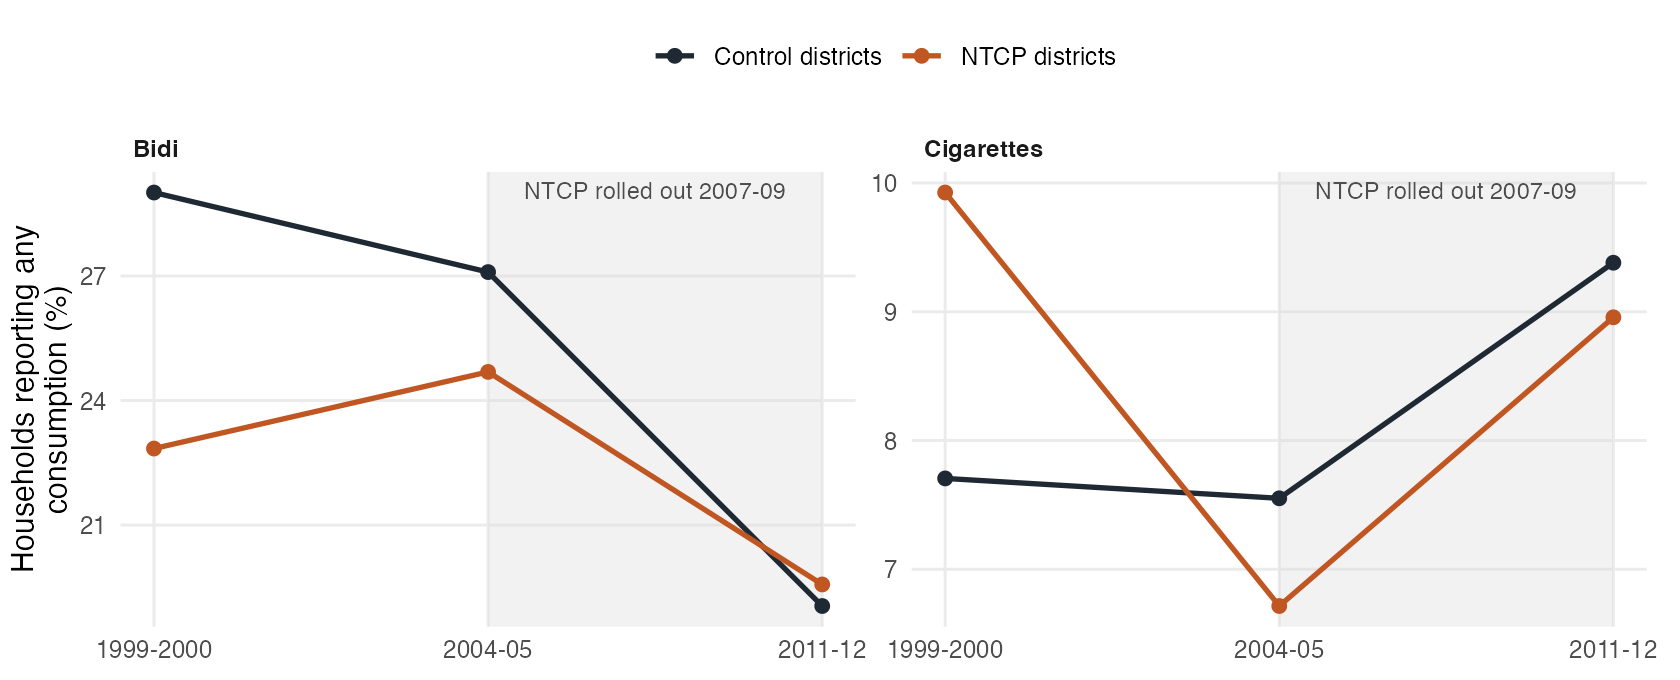
\includegraphics[width=\textwidth]{trends.png}
\caption{Unadjusted prevalence. The shaded band is the 2007--09 rollout.
Parallel trends requires the two lines to be parallel \emph{to the left of}
the band. For bidi they are not: they converge before the programme begins.}
\label{fig:trends}
\end{figure}

% ---------------------------------------------------------------------------
\qhead{Q4. The difference-in-differences by hand}

\begin{lstlisting}[style=rcode]
cell <- tapply(ntcp$any_bidi, list(treated = ntcp$ntcp, year = ntcp$year), mean)
round(100 * cell, 2)

chg_t <- cell["1", "2011-12"] - cell["1", "1999-2000"]
chg_c <- cell["0", "2011-12"] - cell["0", "1999-2000"]
round(100 * c(change_treated = chg_t, change_control = chg_c,
              DiD = chg_t - chg_c), 2)
\end{lstlisting}

\begin{lstlisting}[style=rout]
       year
treated 1999-2000 2004-05 2011-12
      0     29.01   27.09   19.05
      1     22.84   24.69   19.57
change_treated change_control            DiD
         -3.27          -9.96           6.69
\end{lstlisting}

Bidi prevalence fell 3.3 percentage points in NTCP districts and 10.0 points
in control districts. The difference-in-differences is $+6.7$ points.

Read literally, the NTCP districts did \emph{worse}: they failed to fall as
fast as the rest of the country. Nobody should read it literally. Q3 showed
the two groups were already diverging before 2007, and a DiD cannot separate
a pre-existing divergence from a programme effect --- it attributes all of it
to the programme.

% ---------------------------------------------------------------------------
\qhead{Q5. The same number as a regression}

\begin{lstlisting}[style=rcode]
m5 <- lm(any_bidi ~ ntcp * t3, data = subset(ntcp, year != "2004-05"))
round(coef(summary(m5)), 4)
\end{lstlisting}

\begin{lstlisting}[style=rout]
            Estimate Std. Error  t value Pr(>|t|)
(Intercept)   0.2901     0.0013 228.8800        0
ntcp         -0.0617     0.0051 -12.1132        0
ntcp:t3       0.0669     0.0083   8.0563        0
t3           -0.0996     0.0019 -53.4696        0
\end{lstlisting}

The interaction \texttt{ntcp:t3} is $0.0669$ --- the 6.69 points of Q4,
exactly. Each coefficient is one piece of the $2\times2$ table: the intercept
is the control group in 1999--2000 (29.0\%), \texttt{ntcp} is the treated-control
gap in the base period ($-6.2$ points), \texttt{t3} is the control group's
change ($-10.0$ points), and the interaction is the differential change.

Note what the standard errors are doing. They are tiny, because this
specification pretends 220{,}000 households are 220{,}000 independent
observations. They are not: treatment is assigned to 21 districts, so the
effective sample size is closer to 21. Q6 fixes this, and the $t$ of 8.06
becomes a $t$ of 1.45.

% ---------------------------------------------------------------------------
\qhead{Q6. All three rounds, with controls and clustered standard errors}

\begin{lstlisting}[style=rcode]
ntcp$cluster <- paste(ntcp$state_code, ntcp$dist_code)
m6 <- lm(any_bidi ~ ntcp + t2 + t3 + ntcp:t2 + ntcp:t3 +
           urban + log(hh_size) + factor(wealth_q) + factor(state_code),
         data = ntcp)
ct6 <- coeftest(m6, vcov = vcovCL(m6, cluster = ntcp$cluster))
round(ct6[c("ntcp", "t2", "t3", "ntcp:t2", "ntcp:t3"), ], 4)
\end{lstlisting}

\begin{lstlisting}[style=rout]
        Estimate Std. Error t value Pr(>|t|)
ntcp     -0.0365     0.0357 -1.0211   0.3072
t2        0.0241     0.0156  1.5497   0.1212
t3       -0.0475     0.0145 -3.2672   0.0011
ntcp:t2   0.0392     0.0500  0.7849   0.4325
ntcp:t3   0.0620     0.0427  1.4501   0.1470
\end{lstlisting}

The point estimate barely moves: 6.2 points against the 6.7 of Q4. Controls
and state fixed effects are not what was driving it.

The standard error moves by a factor of five, from 0.0083 to 0.0427, and
$p$ goes from essentially zero to 0.147. That is the entire change in the
conclusion, and it comes from clustering, not from the controls. With 879
districts and treatment varying only across them, the honest standard error is
five times the naive one.

Also read \texttt{ntcp:t2}, the pre-period interaction: $+0.0392$, which is
63\% of the size of the ``post'' estimate and in the same direction. The
divergence seen in Q3 is still there after controls.

% ---------------------------------------------------------------------------
\qhead{Q7. Part 1 of the two-part model}

\begin{lstlisting}[style=rcode]
g7 <- glm(any_bidi ~ ntcp + t2 + t3 + ntcp:t2 + ntcp:t3 +
            urban + log(hh_size) + factor(wealth_q) + factor(state_code),
          data = ntcp, family = binomial())
ct7 <- coeftest(g7, vcov = vcovCL(g7, cluster = ntcp$cluster))
or <- function(ct, r) {
  e <- ct[r, 1]; se <- ct[r, 2]
  round(c(OR = exp(e), lo = exp(e - 1.96 * se), hi = exp(e + 1.96 * se),
          p = ct[r, 4]), 3)
}
rbind(DID1 = or(ct7, "ntcp:t2"), DID2 = or(ct7, "ntcp:t3"))
\end{lstlisting}

\begin{lstlisting}[style=rout]
        OR    lo    hi     p
DID1 1.201 0.675 2.135 0.533
DID2 1.400 0.835 2.347 0.201
\end{lstlisting}

DID2 is an odds ratio of 1.40, 95\% CI $[0.84, 2.35]$, $p = 0.20$. No
significant effect of the NTCP on whether a household consumes bidi. The
paper reports 1.03 $[0.84, 1.28]$ --- the same null, with a tighter interval,
because it has twice the treated districts and uses survey weights.

% ---------------------------------------------------------------------------
\qhead{Q8. Part 2, among consuming households}

\begin{lstlisting}[style=rcode]
cons <- subset(ntcp, any_bidi == 1)
cons$lbidi_pp <- log(cons$bidi_sticks / cons$hh_size)
m8 <- lm(lbidi_pp ~ ntcp + t2 + t3 + ntcp:t2 + ntcp:t3 +
           urban + log(hh_size) + factor(wealth_q) + factor(state_code),
         data = cons)
ct8 <- coeftest(m8, vcov = vcovCL(m8, cluster = cons$cluster))
round(ct8[c("ntcp:t2", "ntcp:t3"), ], 4)
\end{lstlisting}

\begin{lstlisting}[style=rout]
        Estimate Std. Error t value Pr(>|t|)
ntcp:t2  -0.0915     0.2073 -0.4415   0.6588
ntcp:t3  -0.0640     0.1408 -0.4541   0.6497
n_consuming
      87465
\end{lstlisting}

DID2 is $-0.064$, so about 6\% fewer bidis per person in NTCP districts after
the programme, with a confidence interval of $[-0.34, 0.21]$ --- comfortably
containing zero. The paper's $0.07$ $[-0.13, 0.28]$ is the same null with the
opposite sign.

On the interpretation: this is a conditional-on-positive estimate, and the
condition is itself an outcome. If the programme pushed some light consumers
to quit, they leave this sample, and the households remaining are the heavier
ones --- which pushes the coefficient \emph{up} even if the programme worked.
So this coefficient is not ``the effect on quantity consumed'' for a fixed
population; it is the effect on quantity among whoever still consumes, a group
the treatment may itself have reshaped. That selection is the price of the
two-part model, and it is why part 1 and part 2 have to be read together
rather than one of them picked.

% ---------------------------------------------------------------------------
\qhead{Q9. The pre-trend test}

DID1 compares 2004--05 with 1999--2000. The NTCP began in 2007. Both periods
therefore precede the programme, so under parallel trends the differential
change between NTCP and control districts should be zero (an odds ratio of 1).
If it is not, the two groups were already diverging and DiD will attribute that
divergence to the programme.

\begin{lstlisting}[style=rout]
   OR    lo    hi     p
1.201 0.675 2.135 0.533
\end{lstlisting}

The test does not reject: $p = 0.533$. Taken at face value, parallel trends
survives.

Now look at the interval rather than the $p$-value: $[0.68, 2.13]$. It is
consistent with the odds of bidi consumption in NTCP districts having fallen
by a third relative to controls, \emph{or} having doubled, before the
programme started. A test that cannot rule out a doubling of the pre-trend
cannot certify parallel trends; it has simply failed to detect a violation.
And the point estimate, 1.20, points the same way as DID2's 1.40.

This is the distinction the exercise is about. ``We tested parallel trends and
it passed'' and ``we had no power to test parallel trends'' produce the same
$p > 0.05$. The raw means in Q3 --- one group rising while the other fell ---
say which of the two this is.

% ---------------------------------------------------------------------------
\qhead{Q10. Cigarettes}

\begin{lstlisting}[style=rcode]
g10 <- glm(any_cig ~ ntcp + t2 + t3 + ntcp:t2 + ntcp:t3 +
             urban + log(hh_size) + factor(wealth_q) + factor(state_code),
           data = ntcp, family = binomial())
ct10 <- coeftest(g10, vcov = vcovCL(g10, cluster = ntcp$cluster))
rbind(DID1 = or(ct10, "ntcp:t2"), DID2 = or(ct10, "ntcp:t3"))
\end{lstlisting}

\begin{lstlisting}[style=rout]
        OR    lo    hi     p
DID1 1.413 0.856 2.332 0.176
DID2 1.795 1.143 2.818 0.011
\end{lstlisting}

DID2 is 1.80 $[1.14, 2.82]$, $p = 0.011$: significant, and in the direction of
\emph{higher} cigarette consumption in NTCP districts. The paper finds 1.01
$[0.82, 1.26]$ --- a clean null.

Resist it. Before this is a finding:

\begin{itemize}[leftmargin=*,itemsep=0.25em]
\item \textbf{21 of 42 treated districts, and not a random 21.} They are the
districts whose names were stable from 1999 to 2011. A district that was split,
renamed or reorganised is a district that was changing, so the selection may
correlate with whatever else was happening there.
\item \textbf{DID1 is 1.41, $p = 0.176$.} Not significant, but 1.41 is most of
the way to 1.80 and in the same direction. The post-programme estimate may
largely be the continuation of a pre-programme trend.
\item \textbf{No survey weights.} The paper uses them; nothing here does. NSS
weights vary a great deal across districts.
\item \textbf{Fewer controls.} The paper also adjusts for religion, caste,
employment type and the age and sex of the household head.
\item \textbf{Round 68 is not strictly comparable.} The 68th round changed the
consumption schedule, a known break in the NSS series, and it supplies the
entire post-treatment period.
\item \textbf{One significant result out of eight tested coefficients.} At
$\alpha = 0.05$ that is about what chance delivers.
\end{itemize}

Any one of these could produce the difference. That is the point: a single
significant coefficient in a replication that departs from the original in six
ways is a question, not an answer.

% ---------------------------------------------------------------------------
\qhead{The write-up}

Three of the paper's four estimates reproduce as nulls; the fourth is
significant here and was not in the paper, under a specification that differs
from the paper's in several ways.

The defensible paragraph is roughly this. This replication is consistent with
the paper's conclusion that the NTCP produced no detectable reduction in
household bidi or cigarette consumption. But it does not establish that the
programme had no effect, and neither does the paper. With 21 treated districts
the confidence intervals admit effects from a one-third reduction to a
doubling of the odds of consumption; the pre-period placebo test is itself too
imprecise to certify parallel trends, and the unadjusted means show the two
groups converging before the programme began. What the data support is that we
\textbf{cannot distinguish} a programme that did nothing from one with a
moderate effect. That is a statement about the evidence, and it is weaker than
``the programme did not work'' --- which is the sentence the design cannot
support.

\begin{notebox}{The habit worth keeping}
Every step that mattered here was a check, not an estimate. Looking at six raw
means before running a regression (Q3). Verifying that the data are not a panel
instead of assuming (Q2). Counting districts within round because codes move
(Q1). Clustering at the level treatment actually varies (Q6). Reading the width
of an interval and not only its $p$-value (Q9). Listing what differs from the
original before believing a result the original did not find (Q10).

The regressions are twenty lines and they were never the hard part.
\end{notebox}

\end{document}
